\section*{Functionel Description Report}
\tableofcontents
\newpage

\section{Abstract}
The projects fundamental goal is to explore and examine properties of 802.11. The focus will be on exploring how management frames can be exploited for malicious use and how this can be mitigated. The main focus is on how deauthentication attacks can lead to Evil Twin Attacks. Further a side focus will be on the different authentication protocols in regards to password cracking. Thus in this project it has been possible to scan and identify the local wireless networks in the area, by exploiting beacon and probe management frames. Hereby giving the ability to deauthenticate clients and emulating a rogue AP for the clients to connect to, hence achieving a man-in-the-middle like state. Lastly it has been possible to crack/obtain a WEP password by obtaining initialization vectors.


\section{Introduction}

Security in wireless networks has become increasingly important do to the rapidly expanding use and need for internet access. However, even with the many security measures in place for wireless networks, there are still vulnerabilities to attacks on said networks. One such attack is the deauthentication attack. Wherein a user will be rejected access to the network he/she is attempting to create a connection to.

This project will, explore the theory and practical applications of deauthentication attacks on networks. Furthermore we will investigate the cracking of passwords used in the encryption of wireless network traffic using the now outdated WEP protocol. To achieve this, we will need to gain knowledge of the wireless local area network (WLAN). Therefore another goal for the project is to create a table of available WiFi's, along with information on clients connected, signal strength etc.

Through this project, we aim to highlight the vulnerabilities of wireless networks and demonstrate the importance of securing them. It is important to note that this project is for educational purposes only and should not be used for malicious activities. Overall, this project will provide a comprehensive understanding of the above-mentioned vulnerabilities of wireless networks and how these might be mitigated/detected.

\iffalse
2 De tre søjler
2.1 Mapping af netværk
    Det skal være muligt at sige alt om sit WLAN:
    • hvor mange WiFi er der (herunder alle AP’s p ̊a hvert WiFi)
    • Hvor mangle klienter findes der (svært ved randomization af MAC (fint teori-afsnit))
    • Hvilken klienter er logget ind p ̊a hvilken netværk
    • Er MAC-adresse en klient eller AP (from-ds/to-ds)
    • Hvor langt/tæt p ̊a er de
    • Hvilke kanaler er meget i brug
    • Evt. s ̊arbarhedsscanning
2.2 Deauth (Evil Twin)
    Det skal være muligt at DoS:
    • Klient
    • AP
    • Kanal
    Ligeledes skal der udforskes, hvorvidt disse DoS kan mitigeres og/eller opdages. god
    at udfolde - henrik Hvis tiden er til det, vil det ogs ̊a være spændende at udnytte deauth til at
    tvinge klienter hen p ̊a et rogue AP (man-in-the-middle).
2.3 Password cracking og WEP/WPA2
    Her opsætter man at man kan bryde den lette password algoritme WEP og ogs ̊a at vise hvordan
    WPA2 forbedrer p ̊a sikkerhden i forhold til WEP. Den bliver meget teoretisk og der skal kommes
    ind p ̊a hvordan WEP og WPA fungerer. Man kan lave nogle matematiske udregninger der viser
    hvor langt tid det gennemsnitligt vil tage at bryde forskellige passwords i WEP og WPA2, som
    tydeligt viser at WPA2 er bedre. Der skal laves kode som bryder pakker med WEP sikkerhed,
    som vi nok selv har lavet, da WEP ikke længere bruges.
\fi

\section{Functionality}
Our project constists of the following functionalities:
\begin{enumerate}
    \item Scan the wireless local access  networks and identify clients/Access Points
    \item Deauthentication attacks
    \item Password cracking
\end{enumerate}

These functionalities aim to be the core of the product that will be created. The first functionality, scanning for local networks, is the most important one as that is the basis of all other functionalities.

A deauthentication attack is a type of denial-of-service attack that targets communication between a user and a WiFi wireless access point \cite{Deauth}. It exploits a feature of IEEE 802.11 wireless networks that allows devices to disconnect from a network by the deauthentication management frame \cite{Deauth_Wiki}.
A deauthentication frame tells a device to stop using the network. It can be sent by either the access point or the device itself. Normally, it is used for legitimate purposes, such as ending a connection or switching to another network.

However, an attacker can exploit this feature and send deauthentication frames to the access point with a spoofed client source address. This causes the spoofed device to lose its connection and try to reconnect. This exploitation has multiple use-cases. If done repeatedly or to multiple devices, this can disrupt or disable the network entirely, thus resulting in a Denial-of-Service (DoS) Attack. Meanwhile it can also be used to obtain a EAPOL 4-way-handshake for WPA or as a way to misguide a client to a rogue access point created by a malicious user to obtain a Man-In-The-Middle state. 

The last point is password cracking. The product should be able to crack basic passwords in the WEP algorithm as that is one of the most basic security algorithms. It is an outdated and non secure algorithm and the product can use some of the multitude of tools available to crack it, such as Aircrack-ng's PTW and FMS or WEPcrack \cite{aircrack-ng}. Alternatively we can create our own algorithm for cracking WEP if the time permit.

The implementations are mainly based on the python library Scapy to implement the functionalities \cite{scapy}. As our network interfaces has to be put in monitor mode a UNIX environment is used. The plan is to use a raspberry pi later in the project to obtain mobility and a uniform platform if time permits. 
The network interface is a Realtek DWA 131-E1 dongle as it is cheap and allows for monitor mode. The UNIX platform has the consequence of limiting the use of the implementation to a specific operating system. Though this should be able to be ported to Windows if need be. Here the Linux-sub-system on Windows might be exploited.
The positive side of using UNIX is that we can implement the program on many types of systems as we use a virtual machine to create the product. Thus making conversion to a raspberry pi easier. The negative side is that we have to use a virtual machine which can create problems with drivers and performance. 

\section{Blocks and sub-blocks}

This project will be built on 3 main blocks, "Mapping of networks", "Deauthentication" and "Password cracking". In in these blocks will be sub-blocks containing functionality for the specific block. 

\subsection{Mapping of networks}
This block takes the physical data being sent in the wireless space, and transforms it into information that the other blocks need and use. It contains a table that holds the information as sub-blocks, for instance access points (AP) in the WLAN, as well as the clients on said AP. Or the signal strength of the AP and which channels are used. This mapping can be done via beacon management frames used by APs to announce their respective presence. Likewise probe management frames can be used to understand what APs a client has been associated with in the past.

\subsection{Deauthentication}
This block handles deauthentication, wherein we deny clients access of certain AP's or all wireless internet usage. Thus making the sub-blocks: 
\begin{itemize}
    \item Client
    \item AP
    \item Channel
\end{itemize}


\subsection{Password cracking and WEP/WPA2}
This block is mainly about WEP and how to crack it, although this also tackles how generally secure passwords are for WEP vs WPA2. There is a high probability that this block also contains some way of creating packets with encryption, as packets with WEP are very uncommon since the widespread release of WPA and beyond.


\section{Theory}
The main theory behind this project is the 802.11 standard \cite{IEEE802.11}. The 802.11 standard, is a set of wireless network protocols developed by the Institute of Electrical and Electronics Engineers (IEEE). The first version of the standard, 802.11, was released in 1997, and since then, several revisions and amendments have been made to improve the technology and increase its capabilities \cite{ETHW}.

The 802.11 standard uses radio waves to transmit data between devices within a wireless local area network (WLAN) without the need for cables or wires. This makes it a popular choice for connecting devices to the internet, especially in homes, offices, and public places such as cafes, airports, and hotels \cite{Public_WiFi}.

Throughout the project, programming will be done mainly in python, using the library Scapy for sniffing, analyzing and transmitting packets. Scapy is a program written in Python, that gives the ability to construct, decrypt, send, capture packets and much more \cite{IEEE_Scapy}. Scapy gives us tools for analyzing 802.11 frames, thus providing the information contained in 801.11 frames. Packets in Scapy are created as objects with layers built on top of each other to define the type of the packet.
\\

\begin{figure}[!htbp]
    \centering
    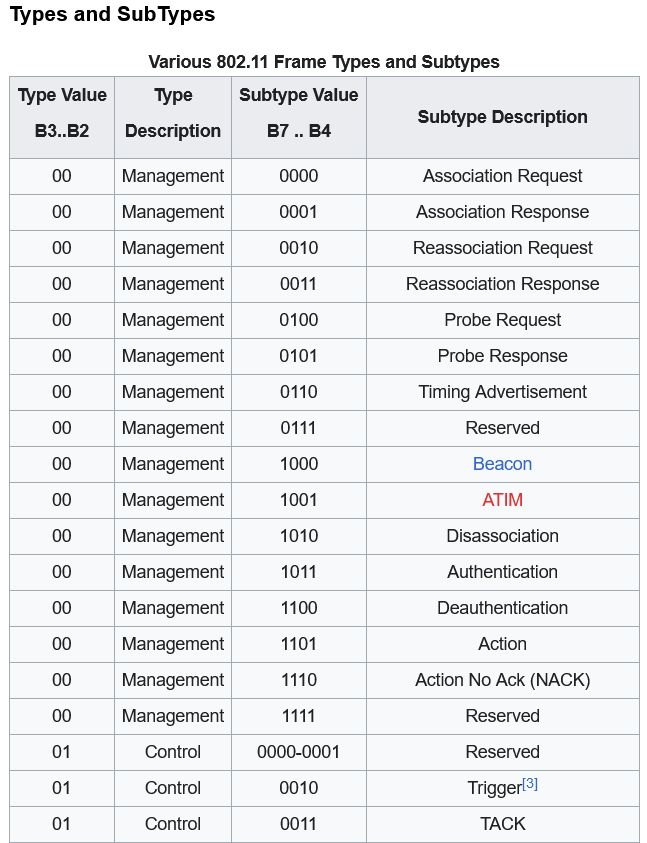
\includegraphics[width=0.5\textwidth]{Latex-Files/Billeder/WIFI_Types.png}
    \caption{WiFi typer og subtyper}
    \label{Wifi Types}
\end{figure}

In 802.11 there are 3 frame types: Management frames, control frames and data frames \cite{Amit802.11frames, DefinitiveGast}. Figure \ref{Wifi Types} shows some of the types and subtypes of different frames with a focus on management frames, since that is what our project is focused on.  Management frames are used by AP's to join and leave the basic service set. They are needed because it is much harder to connect to a specific wireless network rather than a wired network as that is almost automatic when a wire is connected. A wireless network needs to associate a client from a certain sender and ignore others. For clients to know which networks are around them they need to know data about them, this is done via 2 ways of scanning: Active scanning and passive scanning. In passive scanning the client scans every channel passively and listens for beacon frames from AP's, this has the consequence that clients can miss a beacon frame from an AP, since it has to go through every available channel. A beacon frame gives basic information about the AP and are sent continuously by every AP. In active scanning a client sends out probe requests on the channels and listens for probe responses from all the AP's that answer, this has the consequence that a client almost certainly gets information about every single AP in the area. The probe responses gives the client the SSID and capabilities of the AP's. 

Wireless networks also need security while sending packets, i.e. authentication and confidentiality. To ensure confidentiality data frames are encrypted with some sort of security standard. The oldest widespread type being Wired Equivalent Privacy (WEP). It had major security flaws that allows hackers to bypass the algorithm and read the data being sent \cite{WEP1}. Therefore was WiFi Protected Access (WPA) developed in 2003 \cite{WEP3}. 

WEP uses a secret key to encrypt packets between client and AP \cite{WEP2}. The problem with this is that WEP uses the RC4 encryption algorithm, which is known as a stream cipher. A stream cipher operates by making a short key into an infinite random key-stream. The client uses XOR on the key-stream with the plain data to produce the encrypted data. The AP has a copy of the same used key, and uses it to generate an identical key-stream. The AP then uses XOR on the key-stream with the encrypted data to get the exact same plain data back. This type of encryption is easy to misuse, since by flipping a single bit in the encrypted data, the plain data will also have a corresponding single bit flipped. Also the XOR can be found via statistical analysis of key-streams to thereby recover the plain data.

WEP has incorporated defenses against these 2 types of attacks, but they are implemented poorly. The defense against flipping bits are integrity checks in the packet implemented as a CRC-32 checksum. Sadly it is linear which means that it is possible to find the difference between 2 CRC's because the bits that are flipped in the encrypted data is deterministic and therefore an attacker can adjust the checksum and then it is believed that the integrity of the packet is kept, when in reality it isn't.

The defense against the statistical attack is an initialization vector to decrease the chance of reuse of key-streams. The vector is only a 24 bit field and that guarantees the reuse of key-streams. Because of this, the attacker can easily pick up enough data to perform statistical analysis of packets using the same key-stream and then recover the plain data.

WPA2 was a development of the intermediate measure WPA, as a security update to fix many of WEP's problems \cite{WPA2_1}\cite{WEP3}. It was released in 2004 in the 802.11i amendment to the original 802.11. WPA2 uses CCMP protocol which is a development of the AES security algorithm. It rids the network encryption of the previously mentioned security vulnerabilities. 
\\
\begin{figure}[!htbp]
    \centering
    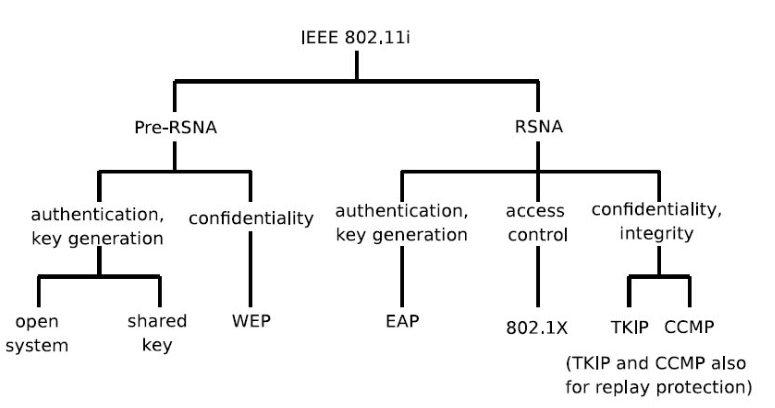
\includegraphics[width=0.6\textwidth]{Latex-Files/Billeder/802.11i security.png}
    \caption{Summary of 802.11i security \cite{WPA2_3}}
    \label{802.11 Security}
\end{figure}

Figure \ref{802.11 Security} shows the different types of securities in the 802.11i standard. It is split up into pre-RSNA and RSNA. Robust
Security Network Association (RSNA) is the way to describe the updated security protocols established with 802.11i and basically means that all security before this standard is out of date. 

For a product to be WiFi certified it requires the usage of a modern security protocol, which is WPA2 \cite{WPA2_2}. New security vulnerabilities have since been found in WPA2 and WPA3 has been created to solve some of those, WPA3 is planned to be implemented widepsread soon. Our focus is not to try decrypting WPA2 or WPA3. 

The authentication of clients and AP's can be exploited by deauthentication attacks. A deauthentication attack is a type of wireless network attack that involves sending forged deauthentication packets to a target client or AP. The theory behind this attack is based on the 802.11 standard, which allows clients to disconnect from an AP using a deauthentication frame.

When a client device is connected to a WiFi network, it sends periodic beacon frames to the access point to maintain the connection. In a deauthentication attack, an attacker sends a series of forged deauthentication packets to the target client or access point, pretending to be the legitimate access point or client. This causes the target to disconnect from the network and require reauthentication, disrupting the communication between the client and the access point.

Deauthentication frames are frames of the management type as seen in figure \ref{Wifi Types}, and have the overall structure as such. Therefore the deauthentication frame contians, among other things, 3 addresses. These three addresses are what can be altered in order to perform a deauthentication attack. One part of the frame body in a deauthentication frame is the reason code, this defines the reason for the termination of the connection. There are 25 different standard reasons defined by Cisco \cite{Cisco_Deathentication_reasoncodes}, these are the ones we will be referring to during the project. Apart from a reasoncode, the frame body includes vendor specific elements, and the Management MIC IE(MMIE) \cite{IEEE_802.11w}. Though this is not always present. The MMIE is only in use when protected management frames are enabled \cite{IEEE_802.11w}. Protected management frames where introduced in order to combat e.g. the deauthentication attack. Since the deauthentication frames are not encrypted in any way, this creates a sizeable vulnerability for a network.

802.11w, realesed in 2009, introduces protected management frames thereby combatting attacks such as deauthentication attacks. This is achieved by ensuring the integrity in the management frame. The integrity check is achieved by the sender calculating a message integriy check(MIC) value, and appending this to the frame. The reciever then calculates the MIC value using the same algorithm, and compares the two. If the two MIC values match, the frame is considered to not having been tampered with, and thus marking it as authentic. Furthermore a frame sequence number(FSN) is introduced, which is used to prevent replay attacks. Replay attacks are not something we will be covering in this project and therefore it wont be analyzed in this report. 

\section{Main Challenges}
Our main challenge in this project is the fact that internet traffic is hard to figure out. There is a lot of data being sent constantly and most of it is not relevant to what we are doing. As we are working with a shared medium it can be hard to differentiate what we are creating and what is part of the standard traffic. Furthermore this makes it difficult to figure out what is going on 'under the hood' when testing our implementations. Thus it has so far taken much longer to perform some of the basic steps of mapping the network and simple deauthentication. Still this is very much a learn by doing project in the way that we obtain solutions to either tackle or overcome the obstacles.

Likewise the theory behind most of the 802.11 management frames and such used in this project is very new to us, since only a short overview of 802.11 has been provided in our courses where the focus mainly has been on the EAPOL 4-way-handshale within WPA. Thus there is a great gap in knowledge we need to fill as some of the implementation parts require a deep understanding of how e.g. the procedure for deauthentication works. 

When we have to decrypt WEP, we have to find some way of getting packets encrypted with WEP, so we either have to find a tool to create WEP packets or find a router that is old enough to be able to create them. 


\section{Time Plan}
In order to generalize and create a overview of our project a timeplan has been created, seen in figure \ref{timeplan}. It is though hard to be sure of what is done when and to give a certain time for each thing. Already now in the process of implementation there has been several obstacles as described in the Main Challenges.  As we are also still early in the process it is still hard to figure out exactly what is needed when and if some of the blocks are even possible to do. 
\\
\begin{figure}[!htbp]
    \centering
    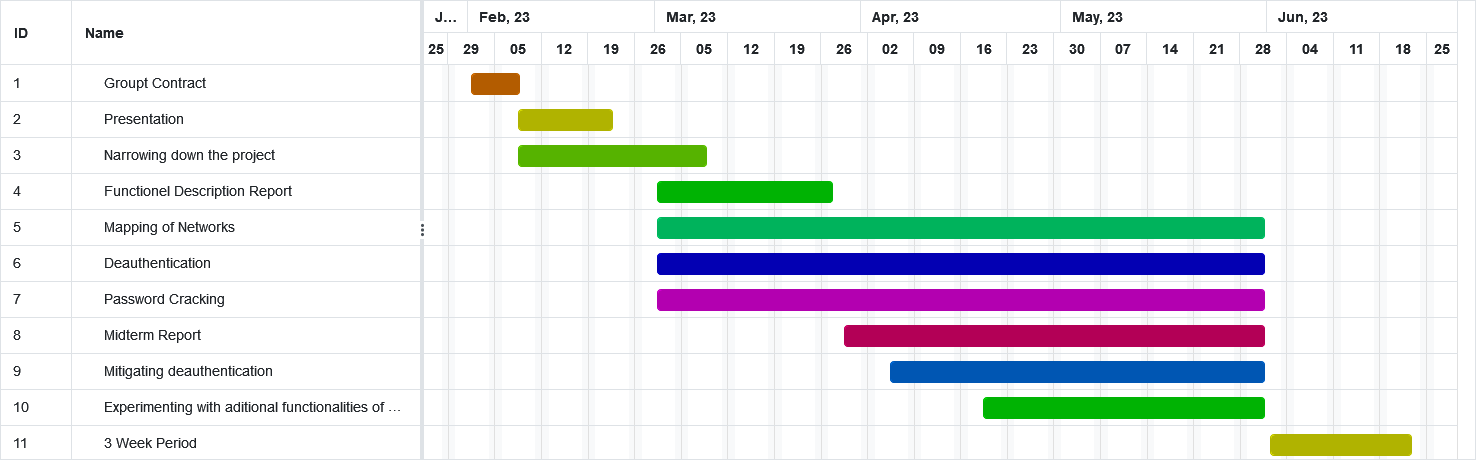
\includegraphics[width=1\textwidth]{Latex-Files/Billeder/Timeplan.png}
    \caption{Timeplan}
    \label{timeplan}
\end{figure}


\section{Conclusion}

We have investigated network traffic via mapping a local WiFi network using Python and the tool scapy to show all AP's connected and sending beacon frames and the clients connected to these networks. We also did deauthentication attacks to disconnect one or more clients from using wireless networking. By doing this we gained advanced knowledge about different types of frames and subframes in the 802.11 standard. We also investigated security in the 802.11 standard, both WEP and WPA2, the 2 most common security algorithms for ensuring the security and integrity of packets and data-streams. Doing this project we also increased our knowledge of python programming and networking toolboxes that use python, which gives a broad understanding of how packets are built in python and in general. 
In the further work on this project, our aim is to gain an even deeper understanding of the processes involved in mapping network, deauthenticating and password cracking. 

